\documentclass[conference]{IEEEtran}
%\documentclass[conference, 10pt]{IEEEtran}
%\usepackage[cp1251]{inputenc}
%\usepackage[russian]{babel}
%\usepackage{pscyr}
\usepackage{graphicx}
\usepackage{cite}

\begin{document}
\title{Test data generation for LRU cache-memory testing}

\author{\IEEEauthorblockN{Evgeni Kornikhin}
\IEEEauthorblockA{Moscow State University, Russia\\
Email: kornevgen@gmail.com} }


\maketitle


\begin{abstract}
System functional testing of microprocessors deals with many
assembly programs of given behavior. The paper proposes new
constraint-based algorithm of initial cache-memory contents
generation for given behavior of assembly program (with cache misses
and hits). Although algorithm works for any types of cache-memory,
the paper describes algorithm in detail for basis types of
cache-memory only: fully associative cache and direct mapped cache.
\end{abstract}

\section{��������}

��������������� �������� ����� �� ������ ������ ��������������
������. ������� ������������ ����������������, � ��� ����� � ��
��������� ������, �������� ���������� �������. ���������
�������������� ������������ ����������� � �������������� ��������
����� �������� �� ����� ���������� (�������� ��������). �����
��������� ����������� � ������ ������, �����������, ������� ��
���������� ��������������� � ����� �������������. � ����������
��������� �������, � ����� ������� �������������� ���� �����
����������� (������������ ��������� ���������, �������� �� ����, ���
�������� � ������������). ������ ��� ���������� ����������
������������ ��� ����������� ���������������� ��������� ���������
�������� ��������, ��� ������ ���������� ������ ��������������
��������� �������� ��������.

� ������~\cite{kamkin} ���������� ��������������� ������� ����������
�������� �������� �� ������ ������ ���������������. � ������ ����
������� ������� �������� ��������� �������������� �������� �
����������� ���� (� ���� ��������� �������) �- ��� ����������
���������� ����������. �������� ������� ��������� ������������������
����������, ��������� ���������� � ��������� ������������ �������
(��������, ������������, ������� ��� ��������� � ���-������). �
�������� ���������� ���������� ����� ���� ������� �������� �
���������. ������������������ ���������� ���� ����� ������ ����.
������������� � �������� ������� ������ ��������� �����, �����
������������ ���������� ���������� ������� � ��� ���� ��������
������������������� ����������, ������ �� ������� ������ ����
��������� �������� �������.

����� �������� �������� ��������� �� ��������� ��������� �������,
���������� ����� ��������� �������� ��������� � ��� ����� ���-������
� ������ ���������, � �������� �������� ���������� �������.
����������� � ������� ������ ���������� ��������� �������, � ������
�� ���������� � ������� ��������� �������� ������. �� ��������
������ �������� ����� ���������� ������������� ���������������
(�������� �������� � ��������, ��� � �.�.), ������� ����������� �
������ ��������� �������. ���������� ����� ������� ��������
��������� ����� ��������� � ���������, ��������� �� ��������� ������
���������� � ���, ��� ���� �������� � �������� �������. ��� �������
�������� �������� (������� �����������, ������� ������������������
����������) ������ ��������� �������� ������ ���������� ���������
���������, ������� � ��������� ������ ������.


\section{�������� ������� (����� �������� ��������)}\label{scheme}
||����� ��� ������������ �� ������� ������ - ���� �������� �����
�����������|| �������� ��������� ����� ��� $\Pi�=�\pi_{start} \cdot
{\langle \pi_i,�x_i(D_i,�S_i)\rangle}_{i=1,n}�\cdot\pi_{stop}$, ���:
\begin{itemize}
\item $\pi_{start}$ �- \emph{���������������� ���������}: �������� ���������������
����������, ��������������� ��� ������������� ���������������;
\item $\langle \pi_i,�x_i(D_i,�S_i)\rangle$ �- \emph{�������� ������} (i�=�1,��,�n):
    \begin{itemize}
    \item $\pi_i$ �- \emph{��������� ���������� ��������� �����������}:
������������������ ����������, �������������� �������������
��������� ����������� ���������� � ���������� ���������
��������������� ����� ����������� ��������� �����������;
    \item $x_i(D_i,�S_i)$ �- \emph{�������� �����������}:
     ����������� ������������������ ����������:
����� ������������ ���������� ����������� $D_i$, � ��������
��������� ���������� � ��������� ��������������� (����������
���������, ���-������ � ������ ���������) ������������� ������������
$S_i$;
    \end{itemize}
\item $\pi_{stop}$ �- \emph{����������� ���������}: �������� ���������������
����������, ��������������� ��� ���������� ������ ���������������;
\item $n$ �- \emph{������ �������� ���������}: �������� ���������, �����������
����� �������� ����������� � ����� �������� ���������.
\end{itemize}

������ �������� �������� ������� \emph{��������� �����������}.
�������� ����������� ��������������� \emph{�������� ��������}
(����������� ������������������� ����������), \emph{�������������
����� ������������} (��� �������� ������ ���������� ������� �����
�����) � \emph{��������� ����������} (������������� �� ��������
��������� ���������� � ��������� ���������������).

\emph{�������� ��������} ���������� ����������� ������������������
���������� ��� �������� ���������� �������� ���������. ������
��������� ������� ������������� ������� ���������� � ��������
�����������. ���� �������� ������ ��������� �������, ��������� ��
���� ����������: ���������� �������� ADD � ���������� ��������� SUB:
\begin{verbatim}
add ... // �������� ������ ��������� ������� ����������
sub ... // �������� ������ �� ���������� �������� ���������
\end{verbatim}

\subsection{����������� ����� ������������}
������������� ��������� �������� ��������, ��� �������, �� ��������
����������� �������� ������������� ������������ ���������������.
������ �������� �������� ��, ����� \emph{����������� �����
������������} �������������� � ������. �������� ��� �������� ����
������������ ����� ������������: \emph{����������� �� ���������} �
\emph{����������� �� �������}. ����������� �� ��������� ���������� �
���������� ���������, �������������� � �������� ��������� ������
���������� ��������� �����������. ����������� �� ������� ����������
��� ���������� ������ � �������, ����� ��� ���������� �������� �
���������� ��������� (load/store instructions). ����������� ��
������� �������� ������� ������� ��� ���������� \emph{������������
�� �����������}, ������� ������������ �� �� ������ ���������� ���
������������ ������������ ���������, � � ������� ����������� ��
�������� ���� ������� ���������� (���������� � �������������). �����
�������������� ��� ������������� ������������ �� ���������:
\emph{����������� ���� �����������-�������������} (define-use
dependencies), ����� �������� ������� ����� ���������� ��������
������� ��������� ��������� �� ��� ����������, � \emph{�����������
���� �����������-�����������} (define-define dependencies), �����
�������� ������� ����� ���������� ����� �������� �������� ���������
��������� �� ��� ����������3. �������� � ������ ���� ������������,
��������, ����������� ���� �������������-������������� (use-use
dependencies), �� ����� ����������� ������ �� ������ �� ������
������ ���������������.

��� ����������� ������������ �� ��������� ���������� ��� �������
�������. � ������ ������� �������� ����������� ����
�����������-�������������:
\begin{verbatim}
add r1, r2, r3 // ����������� �������� r1
sub r4, r1, r5 // ������������� �������� r1
\end{verbatim}

���������� ADD ���������� ���������� ��������� $r2$ � $r3$ �
��������� ��������� � �������� $r1$. ��������� �� ��� ���������� SUB
���������� ���������� �������� $r1$ �- ��� �������� �� �����������
�������� $r1$ ���������� �������� $r5$ � ��������� ��������� �
�������� $r4$.

� ��������� ������� ����������������� ����������� ����
�����������-�����������:
\begin{verbatim}
add r1, r2, r3 // ����������� �������� r1
sub r1, r4, r5 // ��������������� �������� r1
\end{verbatim}

� ���� ������� ���������� SUB ��������� ���� ��������� � ��� ��
����� �������� $r1$, ��� � �������������� �� ���������� ADD.

����������� �� ������� ������������ ���������� ������
���������������. �������� \emph{����������� �� ����������� �������}
� \emph{����������� �� ���������� �������}. � �������� ��������
������������ �� ������� ����� �������� ���������: ����������
����������� �������, ������������ ���������� ������������;
���������� ���������� ������� ��� ������������� ����������� �������;
��������� � ���� � �� �� ������ ������ ���������� �������; ���������
� ���� � �� �� ������ ���-������.

\subsection{�������� ��������}

��� �������, ���������� ��������������� ����� ��������� \emph{������
����������������}, �� ���� � ����������� �� �������� �������
��������� � ��������� ��������������� ����� ���� ��-�������. ���
����������, ���������� ����������, ��������� ������ ����������������
�������� ��������, � ������� ��������� �� ��� ���� ����������. �����
������ ������� \emph{����� ����������������} ����� ��������������
����� ����� ������ \emph{�������� ��������}.

��� \emph{�������� ���������} ��� ���������� ���������� �����������
�� �������� ������� ��������� � ��������� ��������������� �����
������� ���������� ����������. ���� ������������� �� ���������
����������, � �� ������������������ (�������� ������), �����
���������� �������� �������� ��� ������� � ����� ��� ����� ��������
�������� ��� �������� � ���� ����������. �������� ��������
���������� �� ������ ������� �������� ����������� ��������������� �
��� ������� ������. ������ �������� ��� ���� ��������� ������
����������������, � ���������, �������� �� ����������. ����������
������ �������� ���������� ADD �� ������� ������ MIPS64:
\begin{verbatim}
ASSERT WordValue(GPR[rs]) AND WordValue(GPR[rt]) ;
temp <- ( GPR[rs]_31 || GPR[rs]_{31..0} )
      + ( GPR[rt]_31 || GPR[rt]_{31..0} )
IF temp_32 # temp_31 THEN
    SignalException( IntegerOverflow )
ELSE
    GPR[rd] <- sign_extend( temp_{31..0} )
ENDIF
\end{verbatim}

�������� $temp_{32}�\#�temp_{31}$ ���������� ����� ����������������,
��������������� ���������� $IntegerOverflow$; ������ �����
������������� ����������� ���������� ����������.


\section{��������� �������� ������ ��� ��������� �������������
���-������}

\begin{figure}[h]
\centering
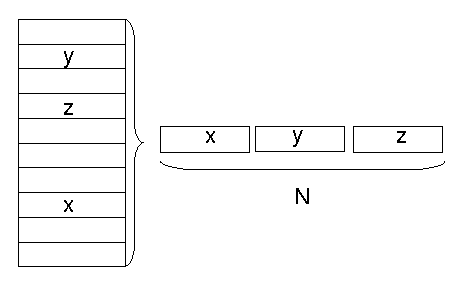
\includegraphics[width=2.5in]{full}
\caption{��������� N-������������� ���} \label{full_assoc}
\end{figure}

\emph{��������� ������������� ���} ������� �� ��������� ����������
����� (�� ���������� ���������� \emph{���������������� ����}). �
������ ������ ���� ����� ��������� ������ ����� ����� ������. ���
������ ���� ������������� ������ ������� ������. ��� ������
���-������ �����������. ��� ��������� � ������ ������ ����� ������
������ � ���� �� ���� ������� ���-������ \emph{�����������}.
�������� \emph{���-���������} ��������, ��� ���� �� ����� ���-������
������������� ���������� ������. �������� \emph{���-�������}
��������, ��� �� ���� �� ����� ���-������ �� �������������
���������� ������. � ������ ���-������� ���� �� ����� ���-������
\emph{�����������} � ���������� �� ������ �� ���������� ������.
�������� ��������� ���������� FIFO (First-In First-Out) �����
��������� ������, ������� ��������� � ���� ������ �����. ����� �����
��� ������ <<����������� ����� $x$>> ����� ���������� �����������
������ �� ������ $x$.

������������ �������� ���������� ����������� ��� ��������� ������� �
������ ��������� ������������� ���-������ ������������ �� ���������
��������� ����������� �������:
\begin{enumerate}
\item ����������� ����� ��� �������� ����� ����� �� ����������
��������� ������� (��� ��������� ����� ������� ���������� ���������
���-������);
\item ����� ����������� ������ � ���-�������� ����� ������ ���������� ���-������� ���� ���������
�������, ������������ � ���� �� ������ ����������.
\end{enumerate}

�������� ������ ����������� �� ��������� ����������:
\begin{enumerate}
\item $\alpha_1, \alpha_2, \alpha_3,...$ --  ������ ����������
��������� ���-������ (�� ���������� ����� ���������������
���-������);
\item ������, ��� ��������� � ������� ���������� ���-��������� (��
���������� ����� ���������� ����������, ��� ��������� � �������
���������� ���-���������);
\item ������, ��� ��������� � ������� ���������� ���-������� (��
���������� ����� ���������� ����������, ��� ��������� � �������
���������� ���-�������);
\item $L_0, L_1, ...$ -- ����������-��������� ���-������
(�� ���������� -- �� ������� ������ ���������� ����������, ���
��������� � ������� ���������� ���-�������).
\end{enumerate}

����, ������ ����������, ��� ��������� � ������� ����������
���-���������, ��������� 1 ����� ����������; ������ ����������, ���
��������� � ������� ���������� ���-������ ��������� 1
����������-��������� ���-������ � 1 ����������-����������� �����.
�������� ��������� ����������� ��� ������ ��������� ����������
��������� ������� ($N$ -- ��������������� ���-������):
\begin{enumerate}
\item <<��������� �����������>> ������������ ��� ������ ������� ���� ���:
$L_0 = \{ \alpha_1, \alpha_2,..., \alpha_N\}$, $|L_0| = N$ (���,
��-�������, ��� ����� $\alpha_1, \alpha_2,..., \alpha_N$ ������);
\item <<����������� ���-���������>> ������������ ��� ������ ����������,
��� ��������� � ������� ���������� ���-���������: $x \in L$, ��� $x$
-- ����� � ����������, $L$ -- ������� ����������-���������
���-������;
\item <<����������� ���-�������>> ������������ ��� ������
����������, ��� ��������� � ������� ���������� ���-������ ($x$ --
����������� �����, $L$ -- ������� ����������-��������� ���-������):
$x \notin L, L' = L \cup \{x\} \setminus \{y\}$, ��� $y$ --
����������� ����� - ��� �����, � �������� ���������� ���-������ �
����������, ����������� ����� ������ ����������� �� $N$ ����������
(� ���� ���������� ��������� ����������). ���� ����� ������
����������� ������ $N$ ����������, �� � ������� ��������� ������� �
��������� ��������� ���������� ��������������� ����� ����������
���������. $L'$ ���������� ������� ����������-��������� ���-������
��� ��������� ����������.
\end{enumerate}

� �������� <<���-��������� ������ $x$>> ��������������� �����
<<���-������� ������ $x$>>, �.�. � ���������� ���-������� ������ ��
����� ������ ������������ � ���, � ������ ������, ������� �����
����������� ��������� ������� � ���� (� ������� <<���������� � ���
���������>>).

���������� ������ ��������� ������� � ���������� ��� ���� ��������
������. ����� ������������� ��� ��� 3-� �������������� ����.

LOAD x, y @ Hit

STORE u, z @ Miss

LOAD z, y @ Hit

������ ����� ����������� � ������� ���������� ���, ����� ��� ��
������ ���� �������� (������ <<������>> ����������). �����, ��� LOAD
���� ����� ������ ����������, ������ ������ ���������� (�.�. � ����
����������� �������� �� ������):

LOAD $x_1, y_0$ @ Hit

STORE $u_0, z_0$ @ Miss

LOAD $z_1, y_0$ @ Hit

������ ���������� ���������� ��������� ���-������: $\{ \alpha,
\beta, \gamma \}$ (�� ���������� ����� ��������������� ���-������).

���� ������ ������� � ������ �������� $x_0, y_0, z_0, u_0, \alpha,
\beta, \gamma$, �� ������� ���������� ��������� ������� �����
��������� � �������� �������� ���������. ������� ������������, ���
������� �� ����� ������������. ��� � ������ ������ ���������� �����
�����-���� ���� �������.

������ ����������� ������� � ��������� ��������� � ��������, ���
�������������� ������� ����������-��������� ���-������:

$y_0 \in \{ \alpha, \beta, \gamma \}$,

$z_0 \notin \{ \alpha, \beta, \gamma \}$,

$y_0 \in \{ \alpha, \beta, \gamma \} \setminus \{ \alpha \} \cup \{
z_0 \}$,

$\alpha, \beta, \gamma$ -- ��� ������

�������� ���������� ������� �����������:

$y_0 \in (\{\alpha, \beta, \gamma\} \cap \{ \gamma, \beta, z_0 \})$

$z_0 \notin \{ \alpha, \beta, \gamma \}$,

$\alpha, \beta, \gamma$ -- ��� ������

��� ���������� �� ����� ������� �����������:

$y_0 \in \{\gamma, \beta\}$

$z_0 \notin \{ \alpha, \beta, \gamma \}$,

$\alpha, \beta, \gamma$ -- ��� ������


��������, ��� $x_0$ � $u_0$ ����� �� ��������� ������� -- ��
�������� ����� ���� ������������.

����� ������ �������� 8 ���. ����� ��� ���������� ��������� ��������
�� ������� �� 0 �� 255. �������� ���������� �����������, �����
�������� ����� �������� ��� ���������� (������ �����, ��� �����
�������� �� �������� ������������):

$\gamma = y_0 = x_0 = u_0 = 0$

$\beta = 1$

$\alpha = 2$

$z_0 = 3$

�������� ���������� ��������� ������� � ������ ����������
����������:

��������� �������� ����: [0, 1, 2]

LOAD x, 0 - Hit, �.�. 0 $\in \{0,1,2\}$;

STORE 0, 3 - Miss, �.�. 3 $\notin \{0,1,2\}$; �������� FIFO 3
�������� � ���-������, 2 �� ���� �����������, ����� ���������
���-������ ����� [3, 0, 1]

LOAD z, 0 - Hit, �.�. 0 $\in \{3, 0, 1\}$

��� ���������� ��������� ������� ���� ��������� �������� ���������
�������� ���������.


\section{Test data generation for direct mapped cache}

\begin{figure}[h]
\centering
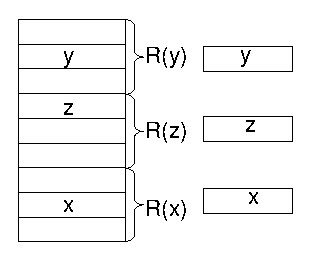
\includegraphics[width=2.5in]{prm}
\caption{Direct mapped cache} \label{prm_pic}
\end{figure}

Whole memory is divided into non-intersecting areas
(\emph{regions}). Direct mapped cache consists of 1 cell for each
region. Each cache cell may store data only from its region. Access
to memory starts from access to cache. \emph{Cache hit} means
successful match cached address with required address in its region.
\emph{Cache miss} means unsuccessful match cached address with
required address in its region. In this case data from cache
replaced by data from memory by required address.

Proposed algorithm generates constraints on the following variables:
\begin{enumerate}
\item $\alpha_1, \alpha_2, \alpha_3,...$ are addresses of the initial
cache state (their count is regions' count);
\item hits-addresses (addresses of instructions from test templates
with cache hit test situation);
\item misses-addresses (addresses of instructions from test templates
with cache miss test situation);
\item evicted addresses (evicted addresses of instructions from test templates
with cache miss test situation);
\item $L_0, L_1, ...$ -- cache states
\end{enumerate}

Define function $R(y)$ which for address $y$ returns a set of all
cells from the same region as region of $y$. $R$ satisfies the
following properties:

$\forall x~( x \in R(x) )$

$\forall x~\forall y~( x = y \rightarrow R(x) = R(y) )$

$\forall x~\forall y~( R(x) = R(y) \leftrightarrow x \in R(y) )$

$\forall x~\forall y~( R(x) = R(y) \leftrightarrow y \in R(x) )$

$\forall x~\forall y~( x \notin R(y) \rightarrow x \neq y )$

Proposed algorithm generates constraints for each instruction by the
following way ($N$ means number of regions):
\begin{enumerate}
\item "initial constraints" are generated one time for each template :
$|\{ \alpha_1, \alpha_2,..., \alpha_N\}| = N$ (other words, numbers
$\alpha_1, \alpha_2,..., \alpha_N$ are different), $|\{ R(\alpha_1),
R(\alpha_2),..., R(\alpha_N)\}| = N$ (other words, all sets
$R(\alpha_1), R(\alpha_2),..., R(\alpha_N)$ are different);
\item "hits-constraints" are generated for each instruction
with cache hit: $x \in L$, where $x$ means address from instruction,
$L$ means a current variable-state of cache memory;
\item "miss-constraints" are generated for each instruction with
cache miss ($x$ means evicting address, $y$ means evicted address,
$L$ means a current variable-state of cache): $y \in L, x \notin L,
L' = L \cup \{x\} \setminus \{y\}, R(y) = R(x)$, $L'$ became the
current variable-cache state for the next instruction.
\end{enumerate}

Constraints for direct mapped cache differ from constraints for
fully associative cache by evicted address constraints only.

Consider test data generation for the already known test template.
Lets memory divided into 3 regions depended on remainder from
division address to 3 (i.e. $R(x) = R(y) \Leftrightarrow 3 | (x-y)$
).

LOAD x, y @ Hit

STORE u, z @ Miss

LOAD z, y @ Hit

Define unique names for variables in test template (each new
variable shouldn't change its value). LOAD gives new version for its
first argument. STORE doesn't generate new version of variables.
Define new variable $z'_0$ for evicted address from the second
instruction (this variable won't be included to the solution):

LOAD $x_1, y_0$ @ Hit

STORE $u_0, z_0$ @ Miss $\rightarrow z'_0$

LOAD $z_1, y_0$ @ Hit

Define variables of initial cache state: $\{ \alpha, \beta, \gamma
\}$ (one for each region).

So the task is looking for values of $x_0, y_0, z_0, u_0, \alpha,
\beta, \gamma$ according to test template. This task has more than 1
solutions. But any solution is enough.

The first constraints describe cache hits and misses as belong to
the current state of cache:

$y_0 \in \{ \alpha, \beta, \gamma \}$,

$z_0 \notin \{ \alpha, \beta, \gamma \}$,

$z'_0 \in \{ \alpha, \beta, \gamma \}$,

$y_0 \in \{ \alpha, \beta, \gamma \} \setminus \{z'_0 \} \cup \{ z_0
\}$,

$R(z_0) = R(z'_0)$,

$\alpha, \beta, \gamma$ -- different

$R(\alpha), R(\beta), R(\gamma)$ -- different

Simplify this constraints set:

$z'_0 \in \{ \alpha, \beta, \gamma \}$,

$y_0 \in \{ \alpha, \beta, \gamma \} \setminus \{z'_0\}$,

$z_0 \notin \{ \alpha, \beta, \gamma \}$,

$ 3 | ( z_0 - z'_0 )$,

$\alpha, \beta, \gamma$ -- different

$R(\alpha), R(\beta), R(\gamma)$ -- different

Note that $x_0$ and $u_0$ don't take part in constraints. So their
values may be arbitrary.

Lets bit length of addresses is 8. So domain of all
variable-addresses is from 0 to 255. Satisfying constraints
variables can get the following values (these values are not
unique):

$\alpha = x_0 = u_0 = 0$

$\beta = y_0 = 1$

$\gamma = 2$

$z_0 = 3$

Verify test template execution with generated initial cache state
and register values:

initial cache state is $L = [(R=0) \mapsto 0, (R=1) \mapsto 1, (R=2)
\mapsto 2]$

LOAD x, 1 - Hit, because $R(1) = L[R=(1~mod~3)]$

STORE 0, 3 - Miss, because $R(3) \neq L[R=( 3~mod~3 )]$, 1 is
evicted from cache, the next state of cache is $L = [(R=0) \mapsto
0, (R=1) \mapsto 3, (R=2) \mapsto 2]$

LOAD z, 0 - Hit, because $R(0) = L[R=(0~mod~3)]$

All instructions from test template were executed according to given
test situations.


\section{���������� ����������� ��� ��������� �������� ������}\label{common_algorithm}

� ������ ������ ������������ �������� ���������� �������� ������
(�.�. ��������� �������� ���������, ����� ���-������, ������
���������� �������, ����� ��� � ��.) ��� �������� ��������. ��������
����������� � ������������ ��������� ����� ���������� �����������
��� ������ ������� � ��������� ����������� �����
�����~\cite{ConstrProp}. ����� �������, �� ��������� ������� �����
��������� ������� �����������, ����� ��� ����� ���������, �
���������� ���� ����� �������� �������� ������.

� ������������ � ��������� ������������ ���������������, �������
��������� ������� � ���������� �������� ��� ���������� � �������, �
������� ����������� ����� ��������� ����������:
\begin{itemize}
\item ������� ����� TLB ��� ������ ���������� ��������� �������
\item ��������� �������� ���������, ��������������� � �������
\item ��������� ��������� �������
\item ����������� ������ ��� ������ ���������� ��������� �������
\item ���� ����� TLB, ��������������� � �������� ��������� (� ������
���� <<r>>, <<vpn/2>>, <<mask>>, <<g>>, <<asid>>, �����)
\item ���� ���������� ������� ��� ������ ���������� ���������
������� (� ������, ���, ���, ������ � ������ ���-������)
\end{itemize}

�������� �� ���������� ���������� ��������������� �������, � ���� ��
�����, ������� ������������� ������������� � �������� ���������. ���
��������� ����������� ��������� ������ ������� �����������.

�������� ����� ����������� � ���� ��������� ������������������
�����:
\begin{enumerate}
\item\label{alg_indextlb} ���������� �������� ����� TLB ��� ������ ���������� ���������
������� �� ������ �������� �������� � ������ TLB (TLB-�������� ���
TLB-���������)
\item\label{alg_testsit} ��������� ����������� �� ��������� �������� ���������, ������
�� �������� �������� ����������, �� ���������� � �������
\item\label{alg_virtual} ��������� �����������-����������� ����������� ������� ��
��������� ��������� ��� ����������, ���������� � �������
\item\label{alg_virtonerow} ��������� ����������� �� ����������� ������, ��������������� �
�������� ������� ����� ������ TLB
\item\label{alg_tlbconsist} ��������� ����������� �� ���� ��������������� � �������� �������
����� TLB, ����������� �������� ��������������� TLB (������
����������� ����� ����� ��������������� �� ����� ����� ������ TLB)
\item\label{alg_physonerow} ��������� ����������� �� ���� ���������� ������� ���
����������, ������������ � ���� ������ TLB
\item\label{alg_cache} ��������� �����������, ������ �� �������� �������� �
���-������ (���-�������� � ���-���������)
\item\label{alg_ozu} ��������� ����������� �� ����������� ������ � ��������
���������, ����������� ������ � ��� (���������� ��������� ��������
���������� ��� ���������� ���������� �������)
\end{enumerate}

������������� ��������� �������� ��, ��� � ���� �����������
���������� <<������������� �����>> ���������� � ������� �� ����, ���
���� �����, ��������, Genesys-Pro: ������ ����, ����� �� ������ ����
(�.�. ��� ������ ��������� ����������) ��������� �������� �������,
���������, �������� (� �������� ��� ���������� ��������),
������������� ����� ���� �������� �� ���������� �������, ���������,
�������� ������ ����������.

���~\ref{alg_indextlb}. ��� ���� -- ��������� ������ ����� TLB, �
������� ���������� ���������� ������ � ������� � �������� �������. �
������ ����� ���� ����� ���������� � ��������� �����������.
����������� ������������ �� ������ �������� �������� � ������ TLB,
��������� � �������. ��������� ����� ����� ���� ��� ���� ��� ����,
��������� ����������� �� ���� ���� ��������� � ����������
����������� �� ����~\ref{alg_cache}. �� ���� ����� ���������� �
�������~\ref{eqs} ������ ������. ���� ���������� � ����������
���������� ����������� ������ ����� �� �������� � ���������� �
���������� ������� ����������� �� ����������� ������ � ��������,
����� �������� ������� � ����� ������ ������� ����� TLB.

��������� ���~\ref{alg_testsit}. ��� ���� -- �������� ����������� ��
��������� �������� ���������, ������ �� �������� ��������
����������, �� ���������� � ������� (��������, ��������������
������������, ������� �� ����). �� ���� ���� ������� ���������� �
�������� ��������������� �������� �������� � ������������� ��� �
����� ����������� ���, ��� ��� �������� ��� ������������ ��������.

���~\ref{alg_virtual}. � ���������� ����� ���� ������ ����������
�����������, ����������� ����������-����������� ������ ���������� �
����������-�������� ���������. ����������� �������� �� ������
�������� �������� �������� ����������, ��� ����������� �����
��������� ����� �� ���������� ��������� AddressTranslation. ��������
����������� ������ ������������ �� ���� ����� �������� ��������,
����������� ����� �� ���������� ����������, � �����������������
��������, ����������� ������ ���������� ����������.

��������� ���~\ref{alg_virtonerow}. � ������ ����� ���� ��� ������
��������������� � �������� ������� ������ TLB ���������� ���
����������� ������ ����������, ���������� � ���� �������.
����������� ������ ���� ����� ���������� �������� ����������
����������:
\begin{enumerate}
\item ����, ��������������� ���� <<r>> ������ TLB, �����������
������� ���������
\item ����, ��������������� ���� <<vpn/2>> ������ TLB, �����������
����� <<mask>> ������ TLB, ���������
\end{enumerate}

���~\ref{alg_tlbconsist} ������� �������� ����������� �� ����
��������������� � ������� ����� TLB � ����� ������� ��������
��������������� TLB (� ������, ��� ������ ����������� ����� �����
��������������� �� ����� ����� ������ TLB): � ����� ���� ����������,
���������� � ������� �������� TLB, ���� ����������� ���� �����
<<r>>, ���� ����������� ���� ����� <<vpn/2>>, ����������� ������
<<mask>> ����� TLB.

�� ��������� ����~\ref{alg_physonerow} ���������� ���������
����������� �� ���� ���������� ������� ����������.
\begin{enumerate}
\item ������������ ���� ���������� ������� -- �������� �������
���������� ������� ��� �������� ������ ����������� �������
\item ������������ ������� � ������� ���-������ ���������� ������� --
�������� ������� ���������� ������� ��� �������� ������ �����������
�������
\item �������� ���������� ������� ����������, ������������ � ����
������ TLB: ���� ���������� ������� ��������� ����� � ������ �����,
����� ��������� ���� �������� ���������� �������� �����������
�������.
\end{enumerate}

���~\ref{alg_cache} ������� �������� ����������� �� ���� ����������
�������, ������ �� �������� �������� � ���-������. �� ���� �����
��������, � ����� ���� ���������� ��� ���������� ��������� �������.
�������� �������� ����������, ������������ � ���� ���, � ��������
��� ��� ����������� ���, ��� ��� ����� ������� � �������~\ref{eqs}.

�������������� ���~\ref{alg_ozu} ������ ����� �������� �����������
�� ����������� ������ � �������� ���������, ������ �� ����������
�������� ����������� ������: ��������, ����������� �� ����������
�������, ���������, ���� ����� ����� �������� �� ����� ������ ��
���� ������; ���� ������ ����, ������� ��������� ����� ������
���������� ��������. ����� ����� (<<$LOAD~x, a$>> -- ����� ����������
������ �� ������, ��� $�$ -- ��������� ��������, $�$ -- ����������
�����; <<$STORE~x, a$>> -- ����� ���������� ������ � ������, ��� $x$ --
������������ ��������, $�$ -- ���������� �����):

\parbox{\textwidth}{
��� ������ $LOAD~x, a_1$ �� �������

\hspace{0.5cm}��� ������ ���������� $LOAD~y, a_2$ �� �������

\hspace{0.5cm}\hspace{0.5cm}����� $a_3, a_4, ..., a_n$ -- ������ � $STORE$ ����� ����:

\hspace{0.5cm}\hspace{0.5cm}�������� ��������� $a_1 \in \{a_2\}\setminus\{a_3,a_4,...a_n\} \Rightarrow x = y$

\hspace{0.5cm}��� ������ ���������� $STORE~y, a_2$ �� �������

\hspace{0.5cm}\hspace{0.5cm}����� $a_3, a_4, ..., a_n$ -- ������ � $STORE$ ����� ����:

\hspace{0.5cm}\hspace{0.5cm}�������� ��������� $a_1 \in \{a_2\}\setminus\{a_3,a_4,...a_n\} \Rightarrow x = y$
}


\section{Conclusion}
The paper devoted to the test data generation problem. Test data
contains initial contents of cache-memory. The paper has proposed
the constraint-based algorithm. Constraints consists of finite sets
variables and sets operations. Test data generation for fully
associative cache and direct mapped cache has been considered in
details. Proposed algorithm is used in projects of testing
MIPS-compatible microprocessors. ECLiPSe is used as constraint
solver.


\begin{thebibliography}{1}

\bibitem{IEEEhowto:kamkin}
A.S.~Kamkin, \emph{Test program generation for microprocessors}
// Proceedings of ISP RAS. \hskip 1em plus
  0.5em minus 0.4em\relax Vol. 14(2). P.23-64. 2008.

\bibitem{IEEEhowto:combinatorial}
K.~Takayama, F.~Fallah, \emph{A new functional test program
generation methodology} // Proceedings 2001 IEEE International
Conference on Computer Design: VLSI in Computers and Processors.
P.76�81. 2001.

\bibitem{IEEEhowto:ATPG}
F.~Ferrandi, D.~Sciuto, M.~Beardo, F.~Bruschi, \emph{An approach to
functional testing of vliw architectures} // Proceedings of the IEEE
International High-Level Validation and Test Workshop (HLDVT�00).
P.29�33. 2000.

\bibitem{IEEEhowto:GenesysPro}
Y.~Lichtenstein, M.~Rimon, M.~Vinov, M.~Behm, J.~Ludden,
\emph{Industrial experience with test generation languages for
processor verification} // Proceedings of the 41st Design Automation
Conference (DAC�04). 2004.

\end{thebibliography}




% that's all folks
\end{document}
